
\documentclass{standalone}

\usepackage{tikz}
\usetikzlibrary{arrows}
\usetikzlibrary{decorations.markings}
\usepackage{pgfplots}
\pgfplotsset{compat=1.14}

\newcommand{\Deltav}{\mathcal{L}}
\newcommand{\gradDelta}[1][w]{\nabla_{#1}\Deltav}

\begin{document}
\pagestyle{empty}
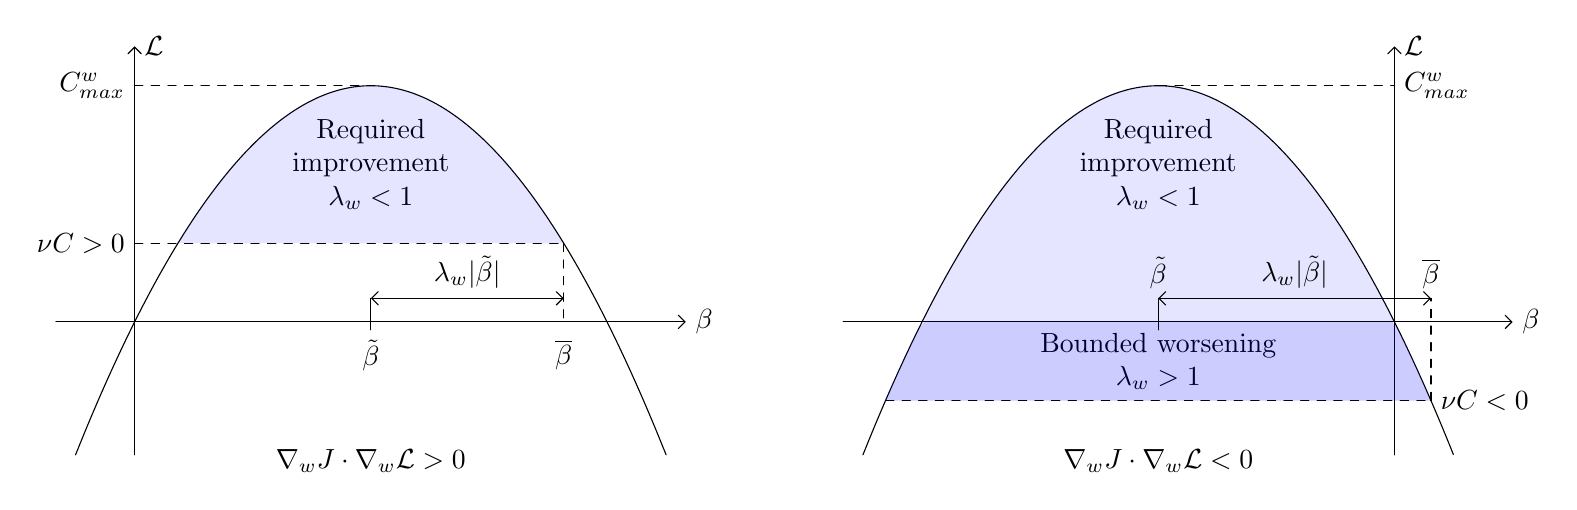
\begin{tikzpicture}[scale=1, line cap=round,line join=round]

\def\xstart{-1}
\def\xend{7}

\def\coeffa{-1/3}
\def\coeffb{2}

\def\domainstart{-0.75}
\def\domainend{6.75}

\def\cone{1}
\def\ctwo{-1}

\def\width{\xend - \xstart}
\def\lowxone{((-\coeffb / 2) - sqrt((-\coeffb / 2)*(-\coeffb / 2) - 4*\coeffa*\cone ))/(2*\coeffa) }
\def\highxone{((-\coeffb / 2) + sqrt((-\coeffb / 2)*(-\coeffb / 2) - 4*\coeffa*\cone ))/(2*\coeffa) }

\def\lowxtwo{((-\coeffb / 2) - sqrt((-\coeffb / 2)*(-\coeffb / 2) - 4*\coeffa*\c2 ))/(2*\coeffa) }
\def\highx2{((-\coeffb / 2) + sqrt((-\coeffb / 2)*(-\coeffb / 2) - 4*\coeffa*\c2 ))/(2*\coeffa) }



% Drawing left image


  \draw[-angle 90] (\xstart,0) -- (\xend,0) node[right] {$\beta$};
  
    \draw[-angle 90] (0,{ \coeffa * (\domainstart * (\domainstart)) + \coeffb*(\domainstart) }) -- (0,3.5) node[right] {$\Deltav$};
  
  \draw[-] ({(\domainend + \domainstart)/2}, 2) node[align=center] {Required \\ improvement \\ $\lambda_w < 1$};
  
  \draw[dashed] (0,{-\coeffb / (2*\coeffa)}) node[left] {$C_{max}^w$} -- (3,{-\coeffb / (2*\coeffa)});
  
  \draw[dashed] (0,1) node[left] {$\nu C > 0$} -- ({3+sqrt(6)},1);
  
  \draw[dashed] ({3+sqrt(6)},1) -- ({3+sqrt(6)},0) node[below, yshift=-0.1cm] {$\overline{\beta}$};


  \draw [domain=-0.75:6.75, samples=50, smooth] plot (\x, {2*\x-(1/3)*\x*\x});
    \draw [draw=none, fill=blue, fill opacity = 0.1, domain={3-sqrt(6)}:{3+sqrt(6)}, samples=100] plot (\x, {2*\x-(1/3)*\x*\x});
    
    
  
  \draw[-] (3,-1.5) node[below] {$\nabla_{w}J \cdot \gradDelta > 0$};
  
  
\draw[-] (3,0.3) -- (3,-0.1) node[below] {$\tilde{\beta}$}; 

\def\highdev{0.3} 
\draw[angle 90 - angle 90] (3,\highdev) -- ({3+sqrt(6)},\highdev) node[midway, above] {$\lambda_w |\tilde{\beta}|$};
  
  
% Second plot  
  
  
\def\highdev{0.3}

  \draw[-angle 90] (9,0) -- (17.5,0) node[right] {$\beta$};
  \draw[-angle 90] (16,{ -1/3 * (-0.75 * (-0.75)) + 2*(-0.75) }) -- (16,3.5) node[right] {$\Deltav$};
  
  \draw[dashed] (13,3)  -- (16,3) node[right] {$C_{max}^w$};
  
 \draw[-] (13, 2) node[align=center] {Required \\ improvement \\ $\lambda_w < 1$};
  \draw[-] (13, -0.5) node[align=center] {Bounded worsening \\ $\lambda_w > 1$};
  
  \draw[dashed] ({10 + 3 - sqrt(12)},-1) -- (16,-1)   -- ({10+3+sqrt(12)},-1) node[right] {$\nu C < 0$};
  
  
  \draw[dashed] ({13+sqrt(12)},-1) -- ({13+sqrt(12)},\highdev) node[above] {$\overline{\beta}$};


  \draw [domain=9.25:16.75, samples=100] plot (\x, {2*(\x-10)-(1/3)*(\x-10)*(\x-10)});

  \draw [draw=none, fill=blue, fill opacity=0.1, domain=10:16, samples=100] plot (\x, {2*(\x-10)-(1/3)*(\x-10)*(\x-10)});  
  
  
    \draw [draw=none, fill=blue, fill opacity=0.2, domain={13-sqrt(12)}:{13+sqrt(12)}, samples=100] plot (\x, {min( 2*(\x-10)-(1/3)*(\x-10)*(\x-10), 0)});  
  
  
  
  
  \draw[-] (13,-1.5) node[below] {$\nabla_{w}J \cdot \gradDelta < 0$}; 
  
  
 \draw[-] (13,-0.1) -- (13,0.3) node[above] {$\tilde{\beta}$}; 

 
\draw[angle 90-angle 90] (13,\highdev) -- ({13+sqrt(12)},\highdev) node[midway, above] {$\lambda_w |\tilde{\beta}|$};
  
 
\end{tikzpicture}

\end{document}